\documentclass{article}[12pt]
\usepackage{graphicx}
\usepackage{amsmath}
\usepackage{indentfirst}
\usepackage{color}
\usepackage{cite}
\usepackage{wasysym}
\usepackage{amssymb}
\usepackage{multirow}
\usepackage{float}



% --Defining Parameters--
\oddsidemargin -0.25in		% Left margin is 1in + this value
\textwidth 6.75in		% Right margin is not set explicitly
\topmargin -0.25in		% Top margin is 1in + this value
\textheight 9in			% Bottom margin is not set explicitly
\columnsep 0.25in		% separation between columns

% -- Change Section Numbers for Roman Numerals -- 
\renewcommand{\thesection}{\Roman{section}} 
\renewcommand{\thesubsection}{\thesection.\Roman{subsection}}
\renewcommand{\figurename}{Fig.}
\renewcommand\refname{REFERENCES}






\begin{document}

\title{Lab 2: Interference of Light}
\author{Samuel Barton}


%--- Heading ---
\begin{center}
\large{\textbf{Laboratory Template}}\\
\bigskip
\small{Samuel Barton}\\
~\\
\small{\textbf{Partner:} Vico Lee; \textbf{Lab Section:} Thursday }\\
~\\
Dated: October 20, 2023\\

\end{center}

%--- Abstract ---
\bigskip
\begin{abstract}
  In this lab was we explored different forms of light interference: two-slit interference and diffraction by a single slit. 
  The objective was to observe the theory about interference with quantitative data.
  Because the observation of light was performed at distances many magnitudes larger than the slit's width, only the Fraunhoger case of diffraction was relevant for this lab.
  We were able to observe the effects of single and double slit(s) on the laser first qualitatively against a clean background, and quantitatively with a light sensor attached to a computer.
  Using the data collected, we calculated the slit width to be $ 1.499\times 10^{-4}~\mathrm{m}$ which was only $ 6.29\% $ off of the actual width of $ 1.6\times 10^{-4}~\mathrm{m}$.
  For the double slit experiment, we found the distance between slits to be $ 2.499 \times 10^{-4}~\mathrm{mm} $, only $ 0.01\% $ off from the reported value.

\end{abstract}
\bigskip

%--- Introduction ---
\section{Introduction}

While in Lab 1 we explored the concept of light as a particle through observation of the photoelectric effect, this lab explored the concept of light as a wave.
This experiment was first performed by Thomas Young in 1801 as a demonstration of the wave behavior of visible light, and in the early 1900s, this experiment was also done with electrons do demonstrate that they exhibit the same behavior.
In this particular experiment, we shined a monochromatic laser ($ \lambda =650~\mathrm{nm} $) through different aperatures.

\begin{figure} [H]
  \center
  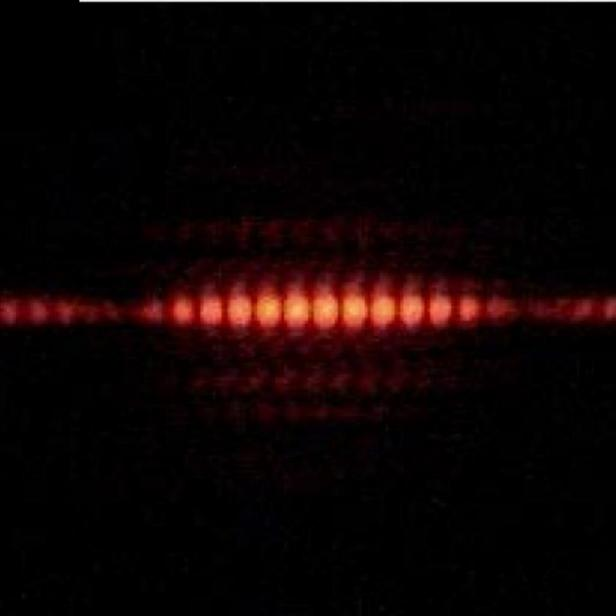
\includegraphics[width=0.45\textwidth]{figures/diffraction_pattern.jpeg}
  \caption{Diffraction Pattern (https://www.discovery.com/science/Double-Slit-Experiment)}
  \label{fig:diff_patt}
\end{figure}

You can seen in Figure \ref{fig:diff_patt} the diffraction pattern upon a screen.
The pattern occurs due to the interference between the EM waves of the visible light.
This effect is due to the diffraction from the small slits: the process causes the light waves to spread out and form wave crests, which then interfere with each other.
When they interfere constructively, we see stronger light intensity, and the peaks observed in the figure.
When they interfere destructively, we see weaker light intensity, and the troughs observed in the figure.

Mathematically, the general diffraction intensity (I) as a function of distance from the center maximum (y) for a single slit is given by:
\begin{equation}
  I(y) = I(0)( \frac{\lambda  r }{\pi y a})^2 sin^2 (\frac{\pi y a }{\lambda  r})
  \label{single_slit_intensity}
\end{equation}
Where $ I(0) $ is the intensity measured on the center maximum, $ \lambda  $ is the wavelength of the EM wave, $ r $ is the distance between the slit and the screen, and $ a $ is the width of the slit.

For the double slit, the intensity distribution is impacted by the interference of the waves from each slit.
This intensity distribution is given by:
\begin{equation}
  I(y) = (\frac{\lambda  r}{\pi y a})^2 \times \sin ^2 (\frac{\pi y a}{\lambda r}) \times 2 [A(r)]^2 \times \cos ^2(\frac{\pi y d}{\lambda  r})
  \label{double_slit_intensity}
\end{equation}
In this experiment, we were able to measure the slit width using equation \eqref{distance} and \eqref{distance2} alongside data we measured. Note that $ a $ is the slit width, $ \lambda  $ is the wavelength, and $ \Delta \theta  $ is the angle between the point of interest on the screen and the maxima of the interference pattern (middle).

\begin{equation}
  \Delta \theta \frac{a}{\lambda } = 1
  \label{distance}
\end{equation}

\begin{equation}
  a = \frac{\lambda }{\Delta \theta }
  \label{distance2}
\end{equation}

We found \eqref{distance} by using \eqref{single_slit_intensity}:
Since Intensity is proportional to $ \sin ^2(\frac{\pi y a}{\lambda r}) $, then we get an intensity of zero when the operand is a multiple of pi.
Thus:
\begin{gather*}
  \frac{\pi y a}{\lambda r} = \pi  \\
  \frac{y a}{\lambda  r} = 1
\end{gather*}
For small angles, $ r \approx D $ and $ \frac{y}{D} \approx \Delta \theta $, thus, equation \eqref{distance} and \eqref{distance2}.

For the double slit, we have \eqref{confusing} where $ \Delta  f_n $ is the distance from the maximum to the n-th minumum, D is the perpendicular distance from the slits to the screen, and n is the n-th minumum diffraction pattern from the middle.

\begin{equation}
  \frac{\Delta  f_n}{\sqrt{\Delta f^2_n+D^2} } = \frac{n \lambda }{d} 
  \label{confusing}
\end{equation}

For the double slit, we can also find the distance between the slits experimentally by using \eqref{dub_slit} which we derived in class.

\begin{equation}
  d = \frac{n \lambda }{\sin \theta }
  \label {dub_slit}
\end{equation}

%--- Method ---
\section{Method}

There were two experiments in this lab: the Manual Exploration and the Quantitative Experiment.
Both used a $ 650(10)~\mathrm{nm} $ laser diode.

\begin{figure}
  \center
  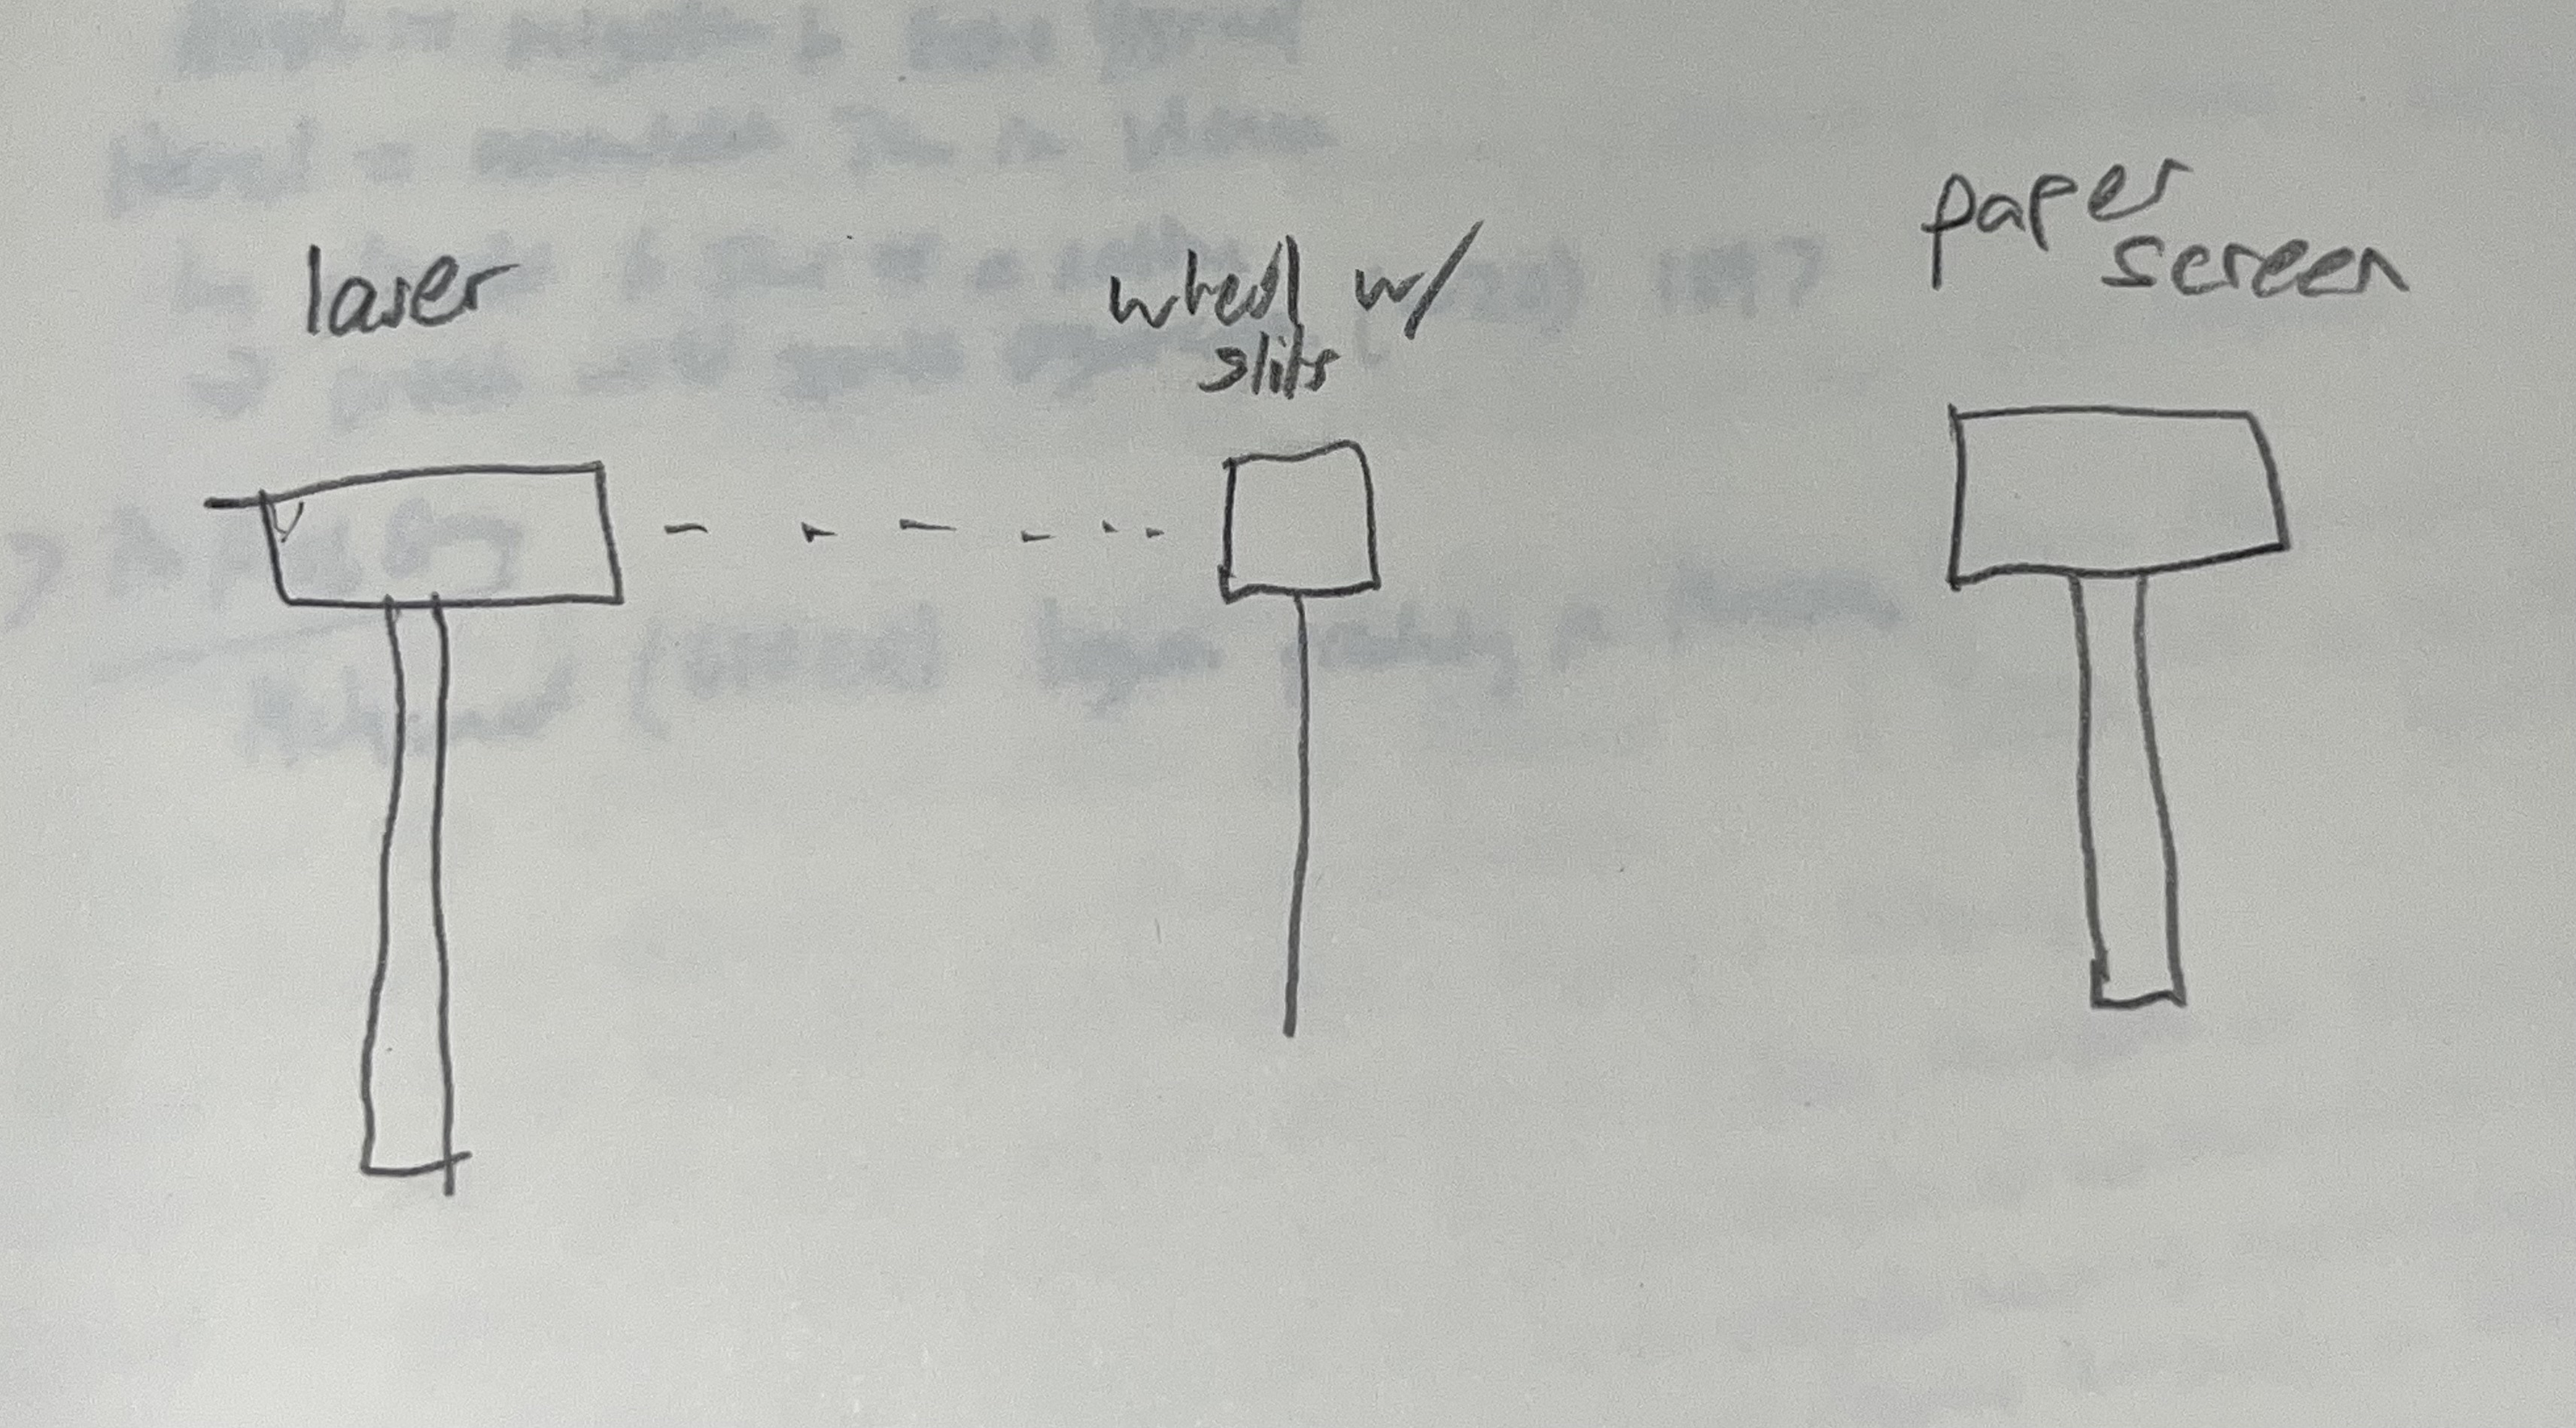
\includegraphics[width=0.45\textwidth]{figures/qual_exp.jpeg}
  \caption{Setup for the Manual Exploration Step}
\end{figure}

\textbf{Manual Exploration}

In this experiment, we observed the diffraction pattern upon a paper screen, and marked down the width of each wave crest.
The screen selector was 31 cm from the slit to maximize the intensity of the light while still seeing the diffraction pattern clearly. 
We used a single slit with width of .08 mm and marked the separation on the paper. 
Then we performed the same process with a dobule slit with the same slit width. 

\textbf{Quantitative Experiment}

\begin{figure}
  \center
  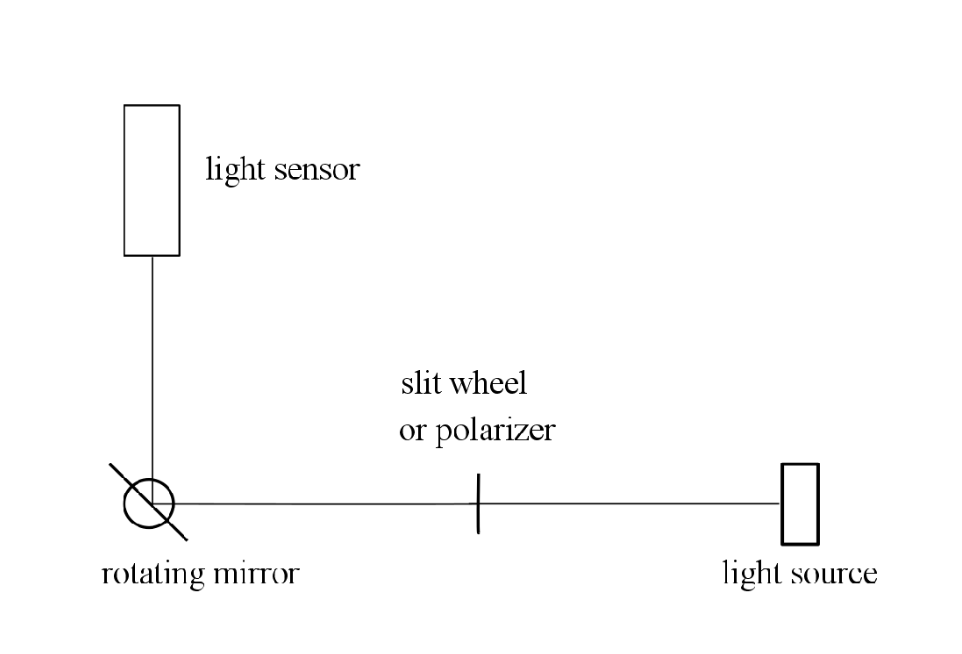
\includegraphics[width=0.45\textwidth]{figures/quant_exp.png}
  \caption{Setup for the Quantitative Experiment}
\end{figure}

In this experiment, we used a light sensor to quantitatively determine the the relative intensities of the bright areas.
After the aperature wheel, we used a mirror to direct the diffracted light beam towards the sensor as seen in the diagram.
The mirror was directed at a constant angular velocity using a motor, and we measured this angular velocity using a timer and a protractor.
For this experiment, we generated four dataplots: two for each the single and double slits, each with different measurement sensitivity.
The two different dataplots with different measurement sensitivities were important because the sensor would saturate out at the point of maximum intensity when it was at its most sensitive.
With the data plot, we were able to observe the difference in relative intensity of the diffraction pattern. 

%--- Data ---
\section{Data, Analysis, \& Results}

\subsection {Single Slit}
\begin{figure}
  \center
  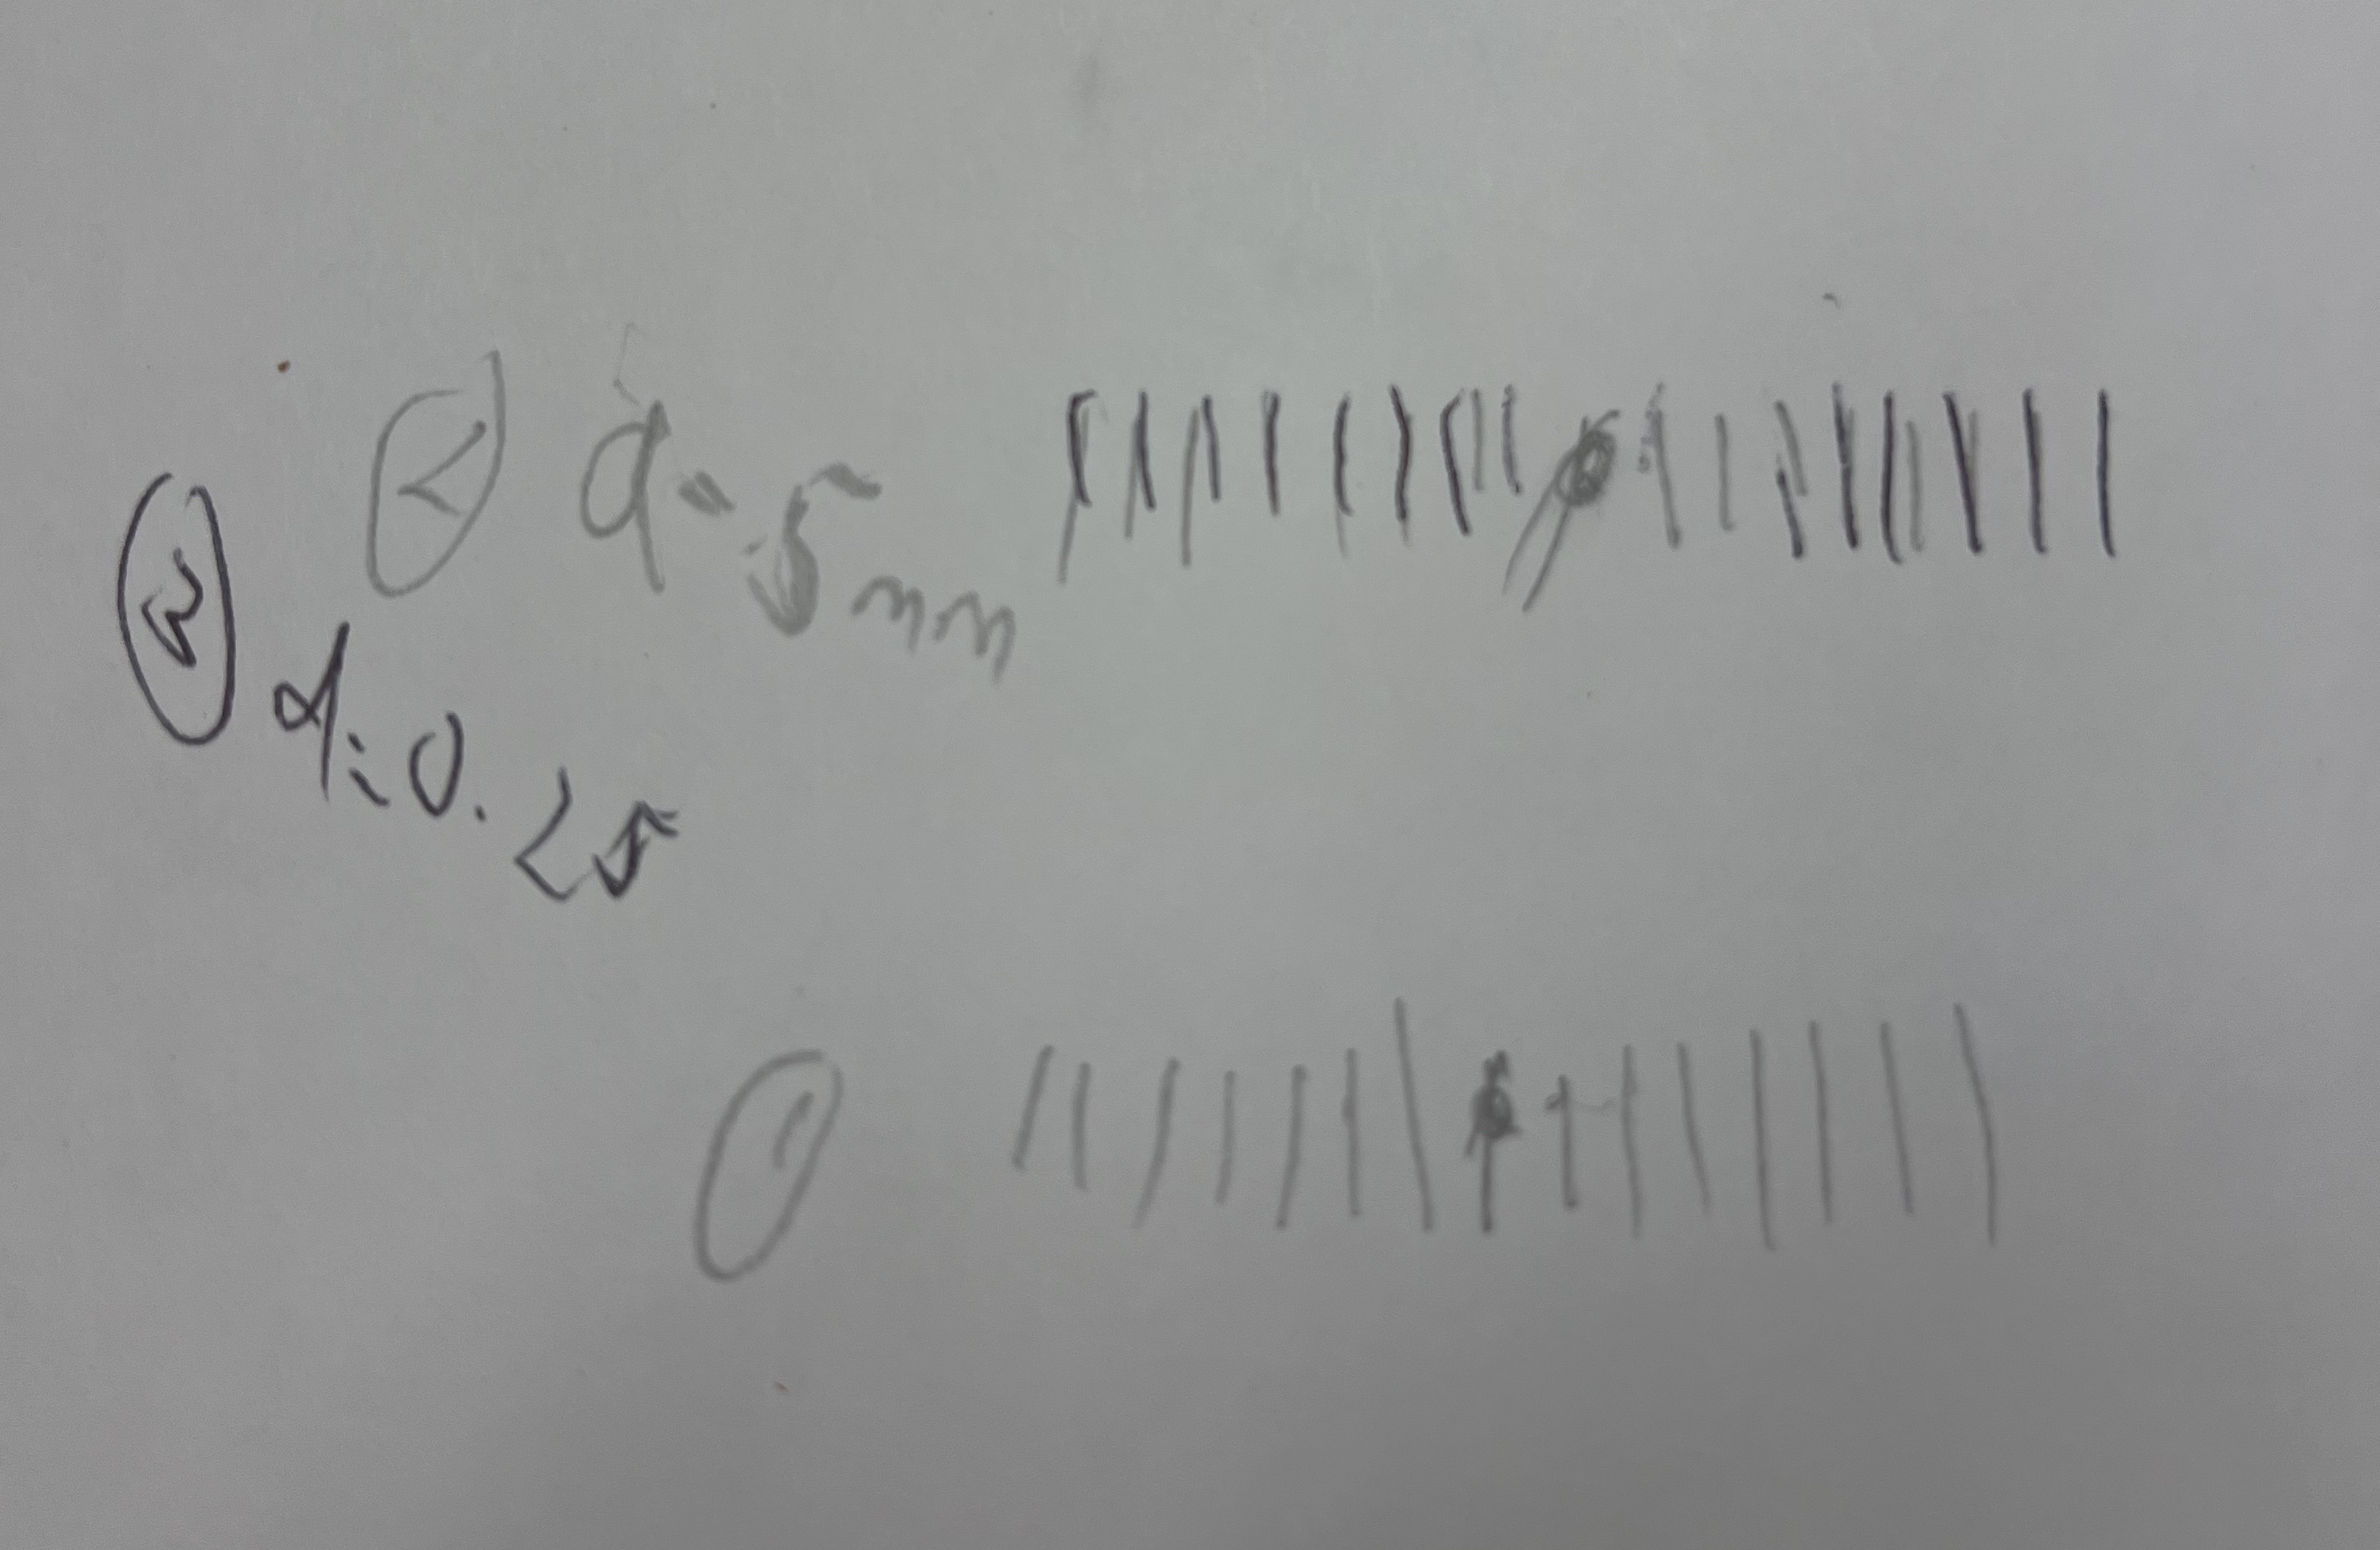
\includegraphics[width=0.65\textwidth]{figures/peaks_drawing.jpg}
  \caption{The Markings of Minima and Maxima from the Manual Exploration Experiment -- (1) represents the minima for a single slit f width $ a = 0.08~\mathrm{mm} $ and (2) represents the minima for a double slit with slitwidth $ a=0.8\mathrm{mm} $ and slit separation $ d=0.5~\mathrm{mm} $. (3) is for double slit with slitwidth $ a=0.8~\mathrm{mm} $ and slit separation $ d=0.25~\mathrm{mm} $}
\end{figure}

For the Manual Exploration, as seen in figure, we found the distance between minima to be $ 1.75 \pm 0.4~\mathrm{mm} $ 
This error range was chosen due to the uncertainty of the human error when marking the maxima and minima, and the uncertainty in the laser itself.
Using \eqref{confusing}, we get $ \Delta f_9  = 12.7~\mathrm{mm}$ or 1.4 mm which is within our expected error range.

\begin{figure}
  \center
  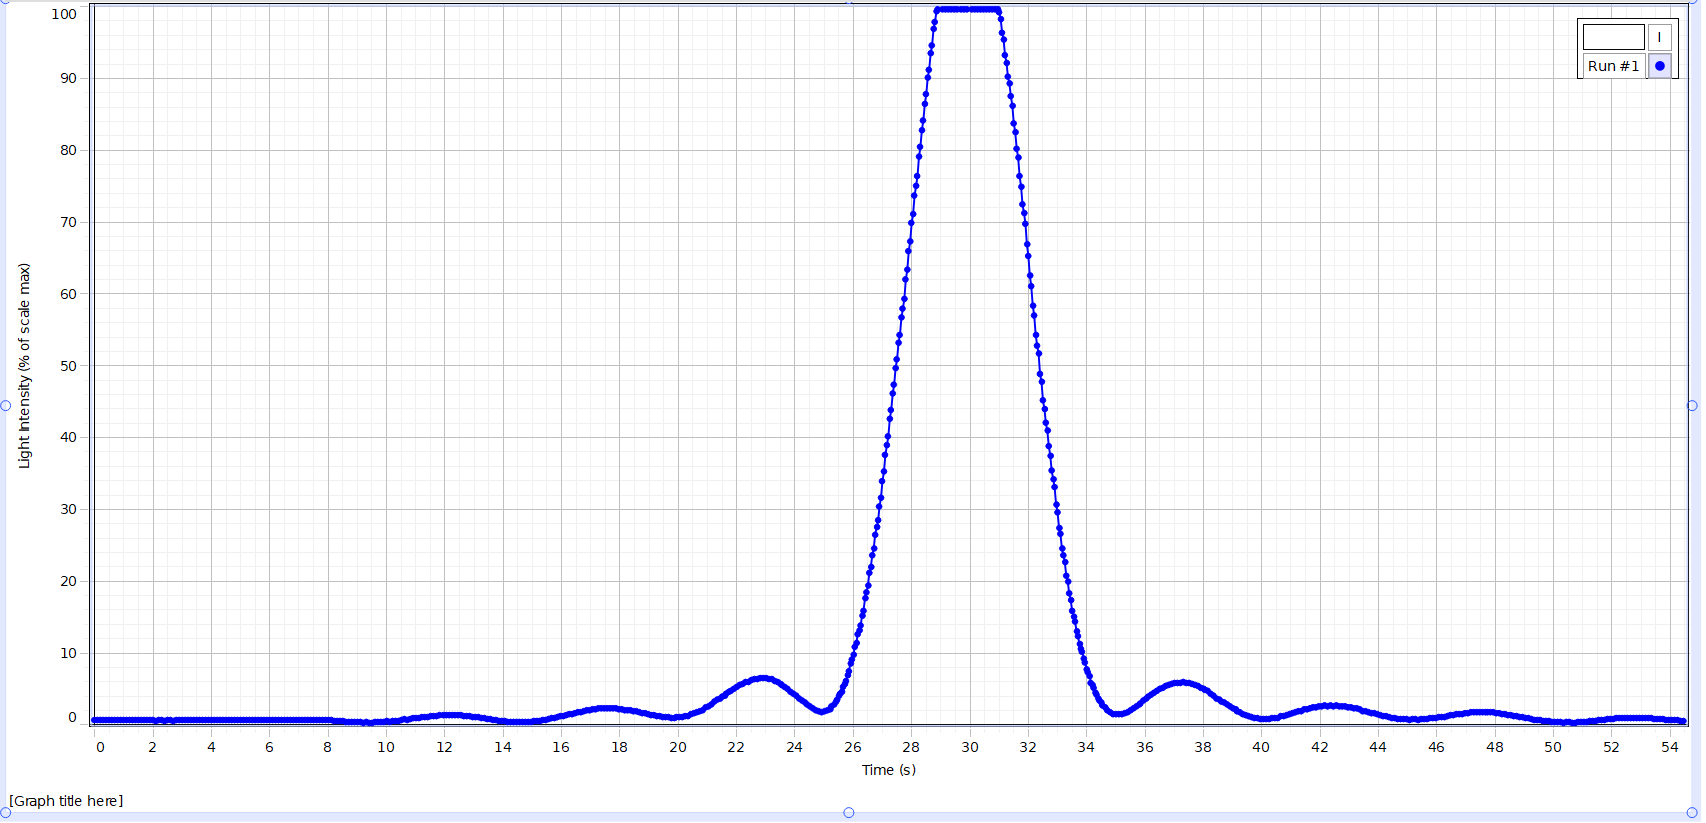
\includegraphics[width=0.65\textwidth]{figures/single_hig.PNG}
  \caption{Single Slit with High Sensitivity}
\end{figure}

\begin{figure}
  \center
  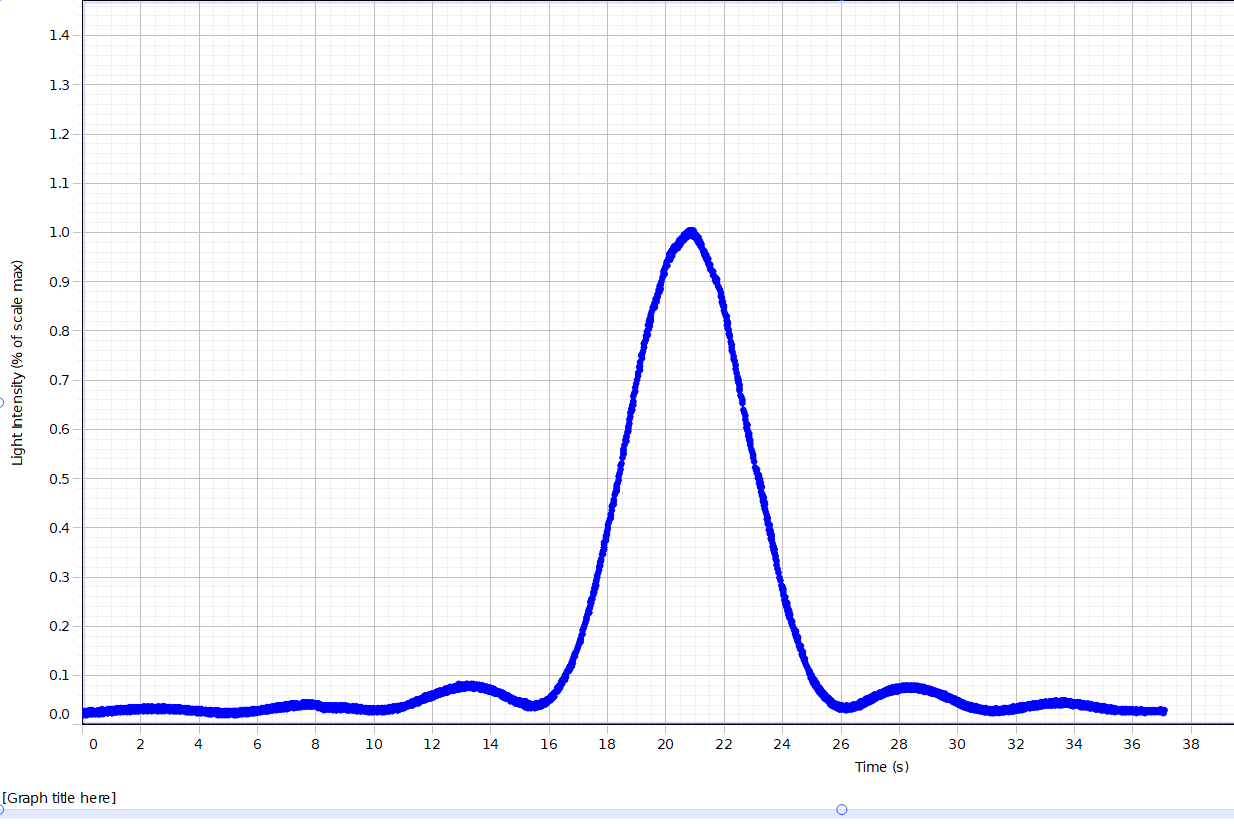
\includegraphics[width=0.65\textwidth]{figures/single_low.PNG}
  \caption{Single Slit with Low Sensitivity}
\end{figure}

For the quantitative experiment, Figures 5 and 6 show the plots of light intensity over time.
Using a protractor and a timer, we measured the 23$ {}^{\circ} $ at 463 seconds yielding in an angular velocity of $ 8.67 \times 10^{-4}~\mathrm{\frac{rad}{s}} $.
We used the plots to find the change in time between minima, $ \Delta t = 5~\mathrm{s} $.
Next, to find $ \Delta \theta  $ we used $ \Delta \theta = \omega \Delta t  $.
Using this quantity in \eqref{distance2}, we found that the slit width, $ a = 1.499\times 10 ^{-4}~\mathrm{mm} $ which has an erorr value from the actual width of .16 mm with a percent error of only $ -6.29\% $.

\subsection{Double Slit}

From the Manual Exploration, the we observed that the patterns for the double slit experiment were quite different from the previous single-slit patterns.
There appeared to be more regions of minima intensity around a narrower region of maximum intensity.
This was expected from looking at \eqref{double_slit_intensity} with the $ \cos ^2 $ and $ \sin ^2 $ factors.
Thus, the intensity would drop to zero whenever
\begin{equation*}
  \frac{\pi y a}{\lambda  r} = n\pi \qquad \text{or} \qquad \frac{\pi y d}{\lambda r} = (M+\frac{1}{2}) m
\end{equation*}
Where $ m $ and $ n $ are whole numbers.
We measured the distance between the minima as shown in Figure 4 to be $ 2.7 \pm 0.3~\mathrm{mm} $. 
Using \eqref{confusing}, we get $ \Delta f_7 = 18.9~\mathrm{mm} $ yielding $ \frac{18.9}{7} = 2.7~\mathrm{mm} $. 
This value aligns with our calculated value.

For the quantitative experiment, Figures 7 and 8 show the plots of relative intensity versus time, mapping out the diffraction/interference pattern, since the mirrior was slowly rotating.
We used the plots to measure the time between troughs, and found this time $ \Delta t = 3~\mathrm{s} $.
With the change in time, we again used the angular velociy previously calculated to find $ \Delta \theta  $.
Plugging values into \eqref{dub_slit}, we get $ d = \frac{650*10^{-9}}{\sin (3*8.67*10^{-4})} = 2.499 \times 10^{-4}~\mathrm{mm} $.
Since the actual distance between the slits is $ 0.25~\mathrm{mm} $, the percent error is $ 0.01\% $.
\begin{figure}
  \center
  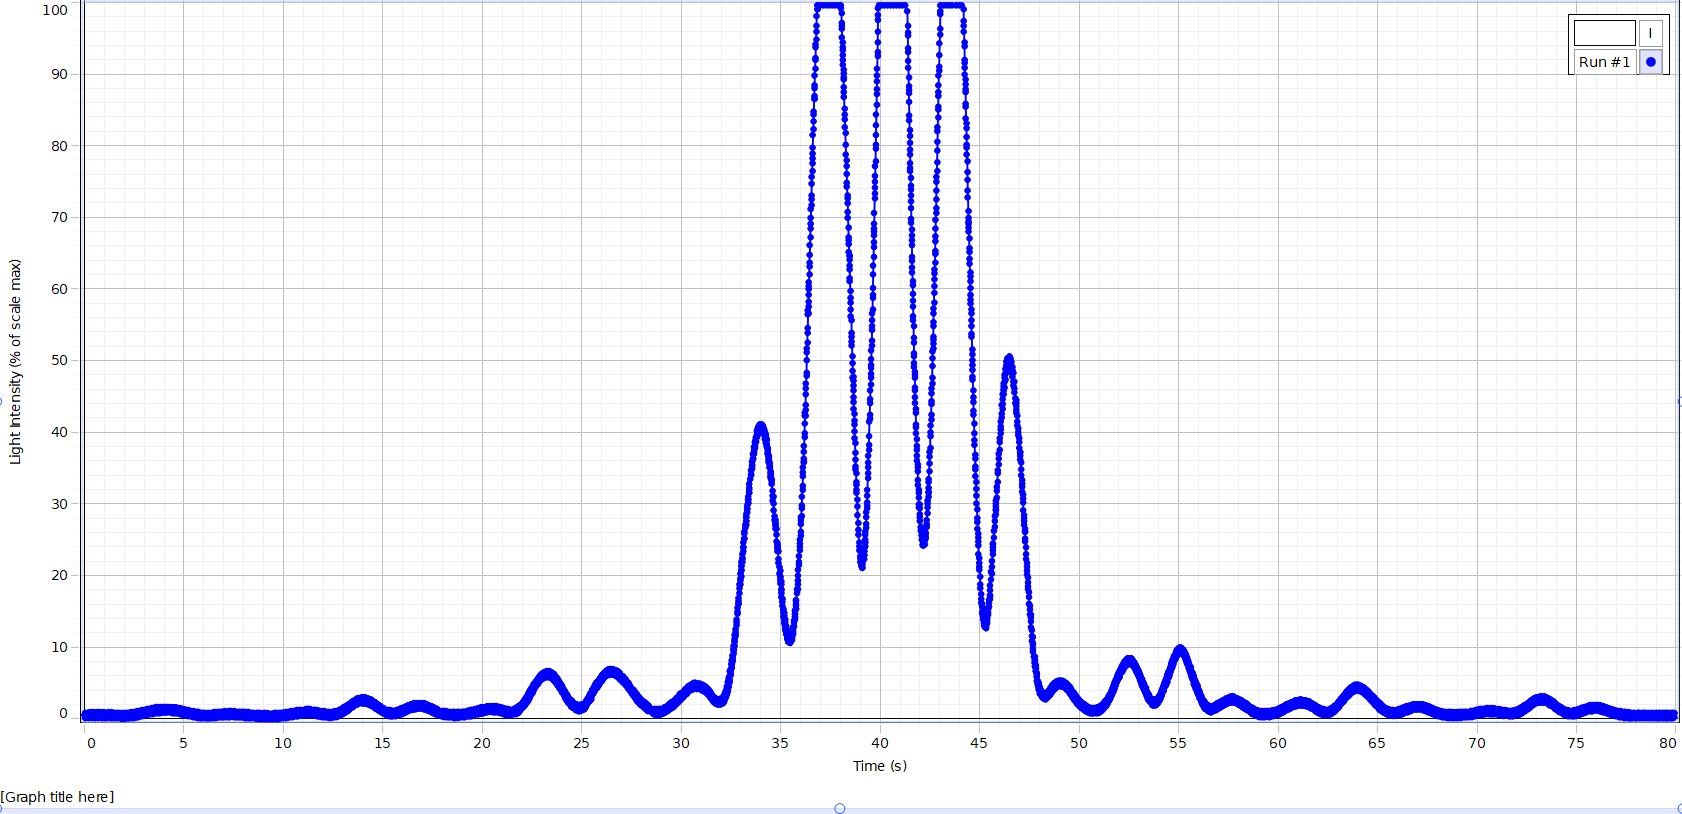
\includegraphics[width=0.65\textwidth]{figures/double_high.PNG}
  \caption{Double Slit with High Sensitivity}
\end{figure}

\begin{figure}
  \center
  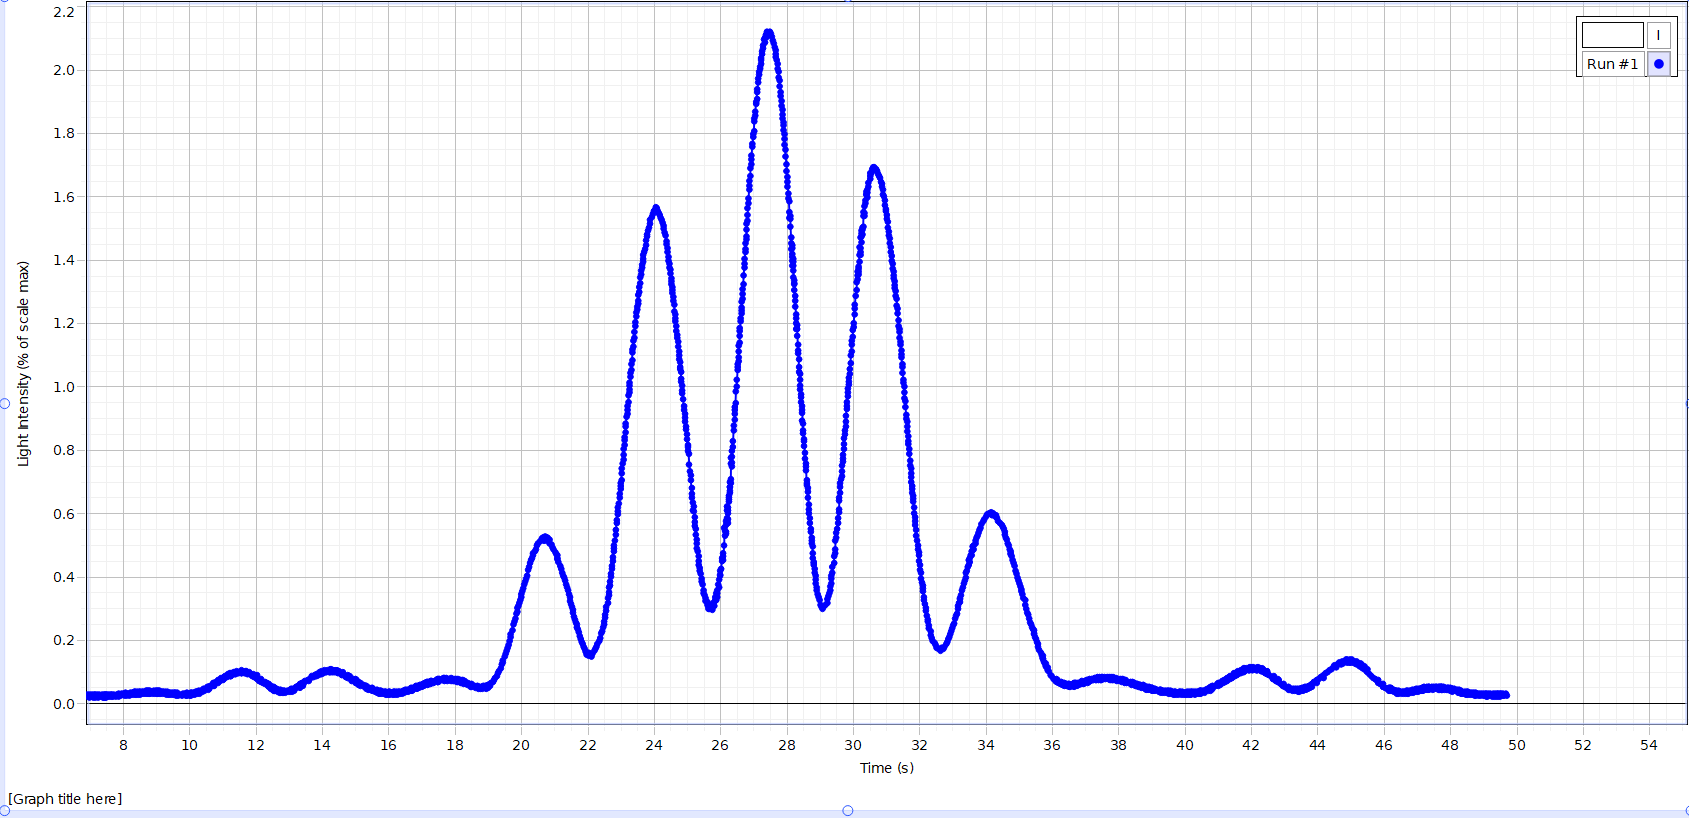
\includegraphics[width=0.65\textwidth]{figures/double_low.PNG}
  \caption{Double Slit with Low Sensitivity}
\end{figure}

%--- Conclusion ---
\section{Conclusion}

In this lab we explored the concept of light as a wave, observing the effects of diffraction and interference. 
We used both a single-slit apparatus to create a diffraction pattern, and a double-slit apparatus to create an interference/diffraction pattern.
The purpose of the lab was to observe the effect of diffraction and interference on the visible light (laser) and we were successful with accurate qualitative and quantitative results.
Combining equations from the Introduction and data from our plots, we were able to theoretically predict the slit-width and slit-distance to high accuracy (under 10\% error) including our degree of uncertainty.



%--- Aknowledgements ---

\end{document}
